\def\micro{\mu m}
\def\um{$\micro$ }
\def\degreesC{$\degree C$ }
\def\percent{$\%$ }
\documentclass[10pt,a4paper,oneside]{article}
\usepackage[left=2cm,right=2cm,top=2cm,bottom=2cm]{geometry}

\usepackage[dvipsnames]{xcolor}

%%  -------------------------------------------------------------------
%%      GDS II layer, regarding MOSIS SCMOS layer map
%%  -------------------------------------------------------------------
% GDS II #41 - P_WELL
\definecolor{pwell}{rgb}{1.0, 0.74, 0.53}   % macaroni and cheese
% GDS II #42 - N_WELL
\definecolor{nwell}{rgb}{0.61, 0.87, 1.0}  % columbia blue
\definecolor{pbase}{rgb}{1.0, 0.51, 0.26}  % mango tango
\definecolor{nbase}{rgb}{0.0, 0.75, 1.0}   % capri 
% GDS II #43 - ACITVE
\definecolor{active}{rgb}{0.9, 0.4, 0.38}   % light carmine pink
% GDS II #45 - N_PLUS_SELECT
\definecolor{nimplant}{rgb}{0.45, 0.76, 0.983}% maya blue
% GDS II #44 - P_PLUS_SELECT
\definecolor{pimplant}{rgb}{1.0, 0.51, 0.26}% mango tango
% GDS II #46 - POLY
\definecolor{poly}{rgb}{0.56, 0.93, 0.56}   % light green
% GDS II #25 - CONTACT
\definecolor{contact}{rgb}{0.83, 0.83, 0.83}% light gray
% GDS II #49 - METAL1
\definecolor{metal1}{rgb}{0.38, 0.31, 0.86} % majorelle blue
% GDS II #50 - VIA1
\definecolor{via1}{rgb}{0.83, 0.83, 0.83}   % light gray
% GDS II #51 - METAL2
\definecolor{metal2}{rgb}{0.04, 0.85, 0.32} % malachite
% GDS II #61 - VIA2
\definecolor{via2}{rgb}{0.83, 0.83, 0.83}   % light gray
% GDS II #63 - METAL3
\definecolor{metal3}{rgb}{0.98, 0.93, 0.37} % maize
% GDS II #30 - VIA3
\definecolor{via3}{rgb}{0.83, 0.83, 0.83}   % light gray
% GDS II #31 - METAL4
\definecolor{metal4}{rgb}{0.75, 0.25, 0.0}  % mahogany
% GDS II #32 - VIA4
\definecolor{via4}{rgb}{0.83, 0.83, 0.83}   % light gray
% GDS II #33 - METAL5
\definecolor{metal5}{rgb}{0.79, 0.08, 0.48} % magenta (dye)
% GDS II #36 - VIA5
\definecolor{via5}{rgb}{0.83, 0.83, 0.83}   % light gray
% GDS II #37 - METAL6
\definecolor{metal6}{rgb}{0.11, 0.35, 0.02} % lincoln green
% GDS II #29 - SILICIDE_BLOCK
\definecolor{silicide-block}{rgb}{0.98, 0.94, 0.9}  % linen
% GDS II #52 - GLASS
\definecolor{glass}{rgb}{1.0, 1.0, 0.88}    % light yellow
% GDS II #26 - PADS
\definecolor{pads}{rgb}{0.75, 1.0, 0.0}     % lime (color wheel)

\definecolor{resist}{rgb}{0.71, 0.4, 0.11}  % light brown

\definecolor{silicide}{rgb}{0.29, 0.33, 0.13}
\definecolor{titanium}{rgb}{0.8, 0.58, 0.46}

\def\OpacityLayout {0.5}

%
% physical
%
\definecolor{substrate}{rgb}{0.96, 0.94, 0.93}  % isabelline
\definecolor{nitride}{rgb}{1.0, 0.03, 0.0}
\definecolor{gateoxide}{rgb}{0.88, 1.0, 1.0}    % light cyan
\definecolor{isolationoxide}{rgb}{0.84, 0.79, 0.87}% languid lavender

\usepackage[utf8]{inputenc}
\usepackage[english]{babel}
\usepackage{forloop}
\usepackage{amsmath}
\usepackage{amsfonts}
\usepackage{amssymb}
\usepackage{gensymb}
\usepackage{mdframed}
\usepackage{graphicx}
\usepackage{tikz}
\usetikzlibrary{arrows,automata,shapes}
\usepackage[siunitx]{circuitikz}
\usepackage{makecell}
\usepackage{array}

\def\WaferClean{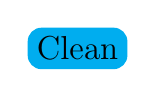
\begin{tikzpicture}\node [fill=cyan, rounded corners=5pt] {\large Clean};\end{tikzpicture}}
\def\WaferSemiClean{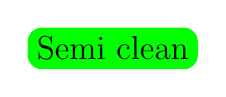
\begin{tikzpicture}\node [fill=green, rounded corners=5pt] {\large Semi clean};\end{tikzpicture}}
\def\WaferNonStandard{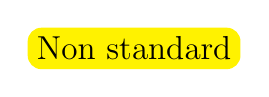
\begin{tikzpicture}\node [fill=yellow, rounded corners=5pt] {\large Non standard};\end{tikzpicture}}

\usepackage[colorlinks=true,linkcolor=blue,urlcolor=black,bookmarksopen=true]{hyperref}
\usepackage{bookmark}
\usepackage{hyperref}
\usepackage{sepfootnotes}
\usepackage{lipsum,tocloft} 
\usetikzlibrary{positioning}
\usetikzlibrary{patterns}

\usepackage{float}
\floatstyle{boxed} 
\restylefloat{figure}

\title{Chemistry essentials for LibreSilicon}
\date{\today}
\author{David Lanzendörfer}
\makeindex

\newcounter{ct}
\def\CrossSectionOnly{0.3}
\def\CrossAndTopSection{0.2}
\def\CrossAndTopSectionBig{0.3}
\def\VLSILayout{0.4}

\DeclareMathOperator\erfc{erfc}

\setlength{\parindent}{0pt} % get rid of annoying indents

\begin{document}
\begin{abstract}
	Copyright © 2017 LANCEVILLE TECHNOLOGY GROUP CO., LIMITED. All rights reserved. \\

This process is licensed under the Libre Silicon public license; you can redistribute it and/or modify it under the terms of the Libre Silicon public license
as published by the Libre Silicon alliance, either version 1 of the License, or (at your option) any later version.

This design is distributed in the hope that it will be useful, but WITHOUT ANY WARRANTY; without even the implied warranty of MERCHANTABILITY or FITNESS FOR A PARTICULAR PURPOSE.
See the Libre Silicon Public License for more details. \\

This document is part of the specification of the free silicon manufacturing standard for manufacturing the LibreSilicon standard logic cells\footnote{\url{https://github.com/chipforge/StdCellLib}} and related free technology nodes from the LibreSilicon project.

For this initial revision 0.1 a gate-first approach has been chosen which led to the choice of polysilicon as the gate electrode material because of the simplicity of the gate alignment.
For better isolation properties of the transistors and gates in overall a box-isolation approach has been chosen.
All of these choices have been made with the future scale down from the recent $1 \mu m$ to smaller structure sizes.
\textbf{This process is for manufacturing $1 \mu m$ only!}
But further releases which will have been tested with smaller structure sizes can be expected.

\end{abstract}

\newpage
\tableofcontents

\maketitle
In this document we deal with all the chemistry related to this manufacturing process.
In case there is anything unclear, please look up this document and its chapters.
We intend to extend this document continuously with all the new recipes we might figure out.
 
\subsection{Etching silicon dioxide}
A very "selective" chemical for SiO2 - i.e. does not etch silicon at all - is hydrofluoric acid (HF). If used directly such etchant has a too fast and aggresive action on the oxide, making very difficult the undercut and the linewidth control. For such reason, HF is universally used as a "buffered" solution, which can keep the etch rate low and constant, by moderating the PH level of the bath. This allows the etching time to be reliably correlated to the etching depth.

The industry standard buffered hydrofluoric acid solution (BHF\label{BHF}) has the following formulation:
\begin{itemize}
	\item 6 volumes of ammonium floride (NH4F, 40\% solution)
	\item 1 volume of HF.
\end{itemize}
This can be prepared, for example, by mixing 113 g of NH4F in 170 ml of H2O, and adding 28 ml of HF.\\
The etch rate at room temperature can range from 1000 to 2500 Å/min (100-250nm/min).
This depends on the actual density of the oxide which, as an amorphous layer, can have a more compact structure (if thermally grown in is oxygen) or less compact (if grown by CVD).
The following etching reaction holds:
\begin{equation}
	SiO_2 + 6HF \rightarrow H_2SiF_6 + H_2O
\end{equation}\\
where $H_2SiF_6$ is water soluble.\\
A common buffered oxide etch solution comprises a 6:1 volume ratio of 40\% NH4F in water to 49\% HF in water. This solution will etch thermally grown oxide at approximately 2 nanometres per second at 25 degrees Celsius.\label{BHF_six_to_one}
\footnote{Wolf, S.; R.N. Tauber (1986). Silicon Processing for the VLSI Era: Volume 1 - Process Technology. pp. 532–533. ISBN 978-0-9616721-3-3} \\

Another popular etching formulation is the P-etch:

60 volumes of $H_2O$ + 3 vol. of HF + 2 vol. of $HNO_3$, that is: 300 ml of $H_2O$ + 15 ml of HF + 10 ml of $HNO_3$.

The P-etch action is strongly dependent on oxide density, as it results from the growth technique.
An example is reported in the literature\footnote{A. Pliskin, J.Vac.Sci Technol., vol. 14, p.1064, 1977}, indicating 120 Å/min for thermal oxide and 250-700 Å/min for sputtered oxide.

A slow etching bath is preferred for opening mask windows for a silicon substrate.
However, the etching process could be used just for removing the oxide film from the whole surface.
In this case the etching speed is not critical, and a fast solution can be used, such as HF diluited 1:10 in water.
The etching time can be easily evaluated by visually inspecting the surface.
Once the oxide film is removed, the metal-grey color of the silicon surface appears.

Sometimes a very light etch is required, for removing just a few atomic layers.
This is the case of surface cleaning and decontamination. HF diluited 1 : 50 in water can be used.
The etching speed will be around 70 Å / min. For example, a typical 50 Å "native" oxide on silicon can be removed with a 45 - 50 sec light etch.

\newpage

\subsection{Etching silicon nitride}
Thin films made of amorphous silicon nitride ($Si_3N_4$) are usually deposited by chemical vapour deposition from silane ($SiH_4$) and ammonia ($NH_3$).
Since they act as a barrier for water and sodium, they have a major role as passivation layers in microchip fabrication.
Patterned nitride layers are also used as a mask for spatially selective silicon oxide growth, and as an etch mask when $SiO_2$ masks cannot be used.

One example of the latter situation is given by the anisotropic etching of silicon in KOH.
The etching rate of $SiO_2$ in KOH is nearly 1000 times slower than the etching rate of silicon, and in most cases a $SiO_2$ mask can be used successfully.
However, a very deep selective etch may require a long etching time, and the 1000:1 etching rate ratio may result still too small to prevent the $SiO_2$ mask from being etched off before the process is completed.
In this circumstance $Si_3N_4$, thanks to its reduced etched rate, can successfully replace the oxide mask layer.

The wet etching of nitride films is often performed in concentrated hot orthophosphoric acid ($H_3PO_4$).
The bath temperature can range from 150°C to 180°C (boiling point) with a corresponding etch rate between 10 and 100 Å/min.
It is good practice to bring the vapours into contact with a cold surface and to drive the condensed liquid back into the etching bath.
This technique is referred to as "reflux".

The etching rates of silicon nitride, silicon oxide, and silicon in $H_3PO_4$ are respectively in the 50 : 5 : 1 ratio.
\newpage
\section{Growing silicon nitride}\label{chemistry_growing_nitride}
In order to grow a high quality layer of silicon nitride on top of a silicon wafer which is adapted to be patterned and to serve as a mask for diffusion or implantation of selected impurities, the wafer is best put into a chamber evacuated to a pressure less than about 1 Torr and heated between 650 and 900 \degree C.
A gaseous mixture comprising primarily of ammonia and a silicon compound, having a ratio of relative concentrations in the range on 4:1 and 20:1 \footnote{\url{http://www.freepatentsonline.com/4395438.html}}, is flooded into that chamber with a silicon compound flow rate of greater than approximately 12 cubic centimeters per minute.
The growth rate will be around 50 Angstroms per minute.
That setup is called Low-Pressure Chemical Vapor Deposition (LPCVD), which is commonly available in basically any semiconductor manufacturing plant or laboratory.


\end{document}